The team worked together as described in the  two following sub-sections: i) Project organisation (structure of the team, where functionality and administrative task were assigned) and ii) Decision making and conflict resolution methodologies (i.e. How we make decisions and solve conflicts or disagreements as a team).

\subsection{Project Organisation}

5.1.1  Roles

All team members have two type of tasks: i) core tasks (e.g. programming goals) and ii) administrative tasks (e.g. documentation. In addition, the coordinator would be the officially communication channel of our team (i.e. our representative). However, it is clarified that this role does not imply a position of leadership or decision making (the decisions are made by the whole group following the decision making and conflict resolution methodology in section 2.4). The specific roles were already stated in the previous section (see Figure 2).

5.1.2.  Communication and work team tools.

\begin{itemize}
	\item Slack (for communication purposes and specific tasks).
	\item GitHub (for code sharing and version control).
	\item Compulsory weekly meeting every Monday (12:00 PM - 2:00 PM).
	\item Compulsory Google Hangout every Sunday (5:00 PM- 6:00 PM).
	\item Extra Google hangout meeting (when needed).
	\item Meeting on Wednesdays 2:00 PM- 5:00 PM (if needed). 
	\item A timetable and advance curve control (i.e. where we are vs where we ought to be).
	\item Our decision-making and conflict resolution methodology (Section 2.4).
	\item Learning meeting (each 15th day we discuss what we can improve as a team)
\end{itemize}


our activities are organised in the client development by hierarchy over the time. Thus, making the text message (which is mandatory) is more important than the image message (which is optional but highly desirable). Considering the above, we divide our horizontal tasks to develop each activity of the previous timetable, as follows.


\begin{figure}[ht]
\centering
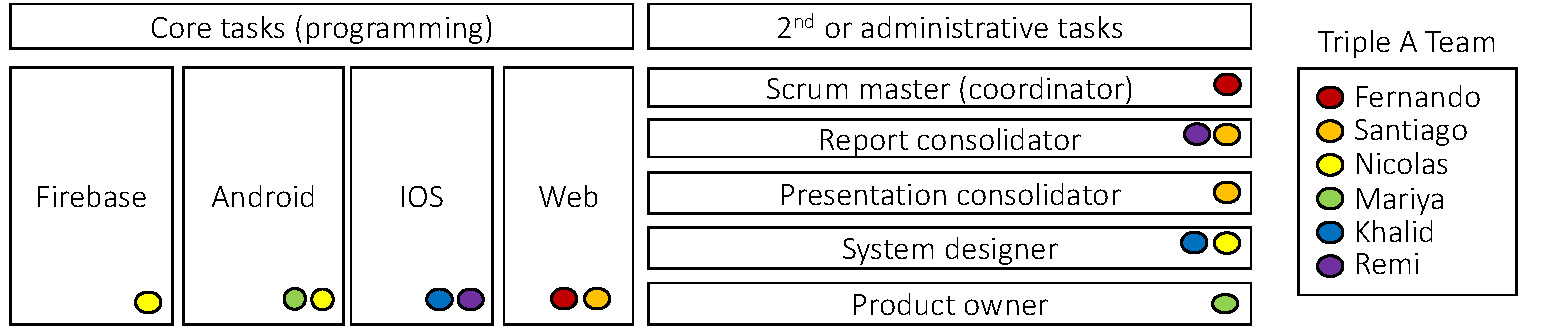
\includegraphics[width=1\textwidth]{figs/tasks}
	\caption{Tasks allocation}
	\label{fig:Tasks}
\end{figure}



5.2. Decision Making and Conflict Resolutions

Making agile agreements and rapidly solve conflicts is a key driver to maximise our team output. Our methodology is inspired in the agents and multiagent theory ~\cite{4646etyet}, specifically in a practical reasoning agent BDI (Belief – Desires - Intentions).

In this manner, each team member always have a valid point of view. Any difference between opinions is a deliberation process (where personal conflict is a conciliation process, which is a special type of deliberation), that would transform a set of options to a set of intentions (this implies that each time there is a deliberation process, the first step is to state a set of options). Then we will plan and assign resources. However, the deliberation process required a balance due to time restrictions (based on our timetable and curve advance). This implies that we must state a mechanism to accelerate the process wherever it is appropriated (deliberation process output is the ideal, but in a practical sense no always we will have time for a full consensus).

So, each time that we can't achieve a full consensus due to time restrictions, we have specified an agreement protocol that precipitated a final decision where the group will be move forward. For this, we use the \footnote{Borda Count: Each option receives $(m-1)$ points for each voter who vote as a first choice, $(m-2)$ for each voter who vote as a second choice, and so on, where $m$ is the number of options.  The winner option is that with more points. If there is a tie the decision will be random.} Borda Count vote procedure, to try to maximise the preferences of all the group.

Finally, for a personal conflict (such as a communication problem), there will be an arbitration protocol to try to solve it. Basically, the team identify those members that are no involving in the conflict in order that they can mediate. If after a conciliation process there is no any agreement, referees will make the decision (only if there are 2 or more referees). If referees declare itself unavailable to reach a final decision, then we will activate the agreement protocol. The following flowchart summarises our methodology.

\begin{figure}[ht]
\centering
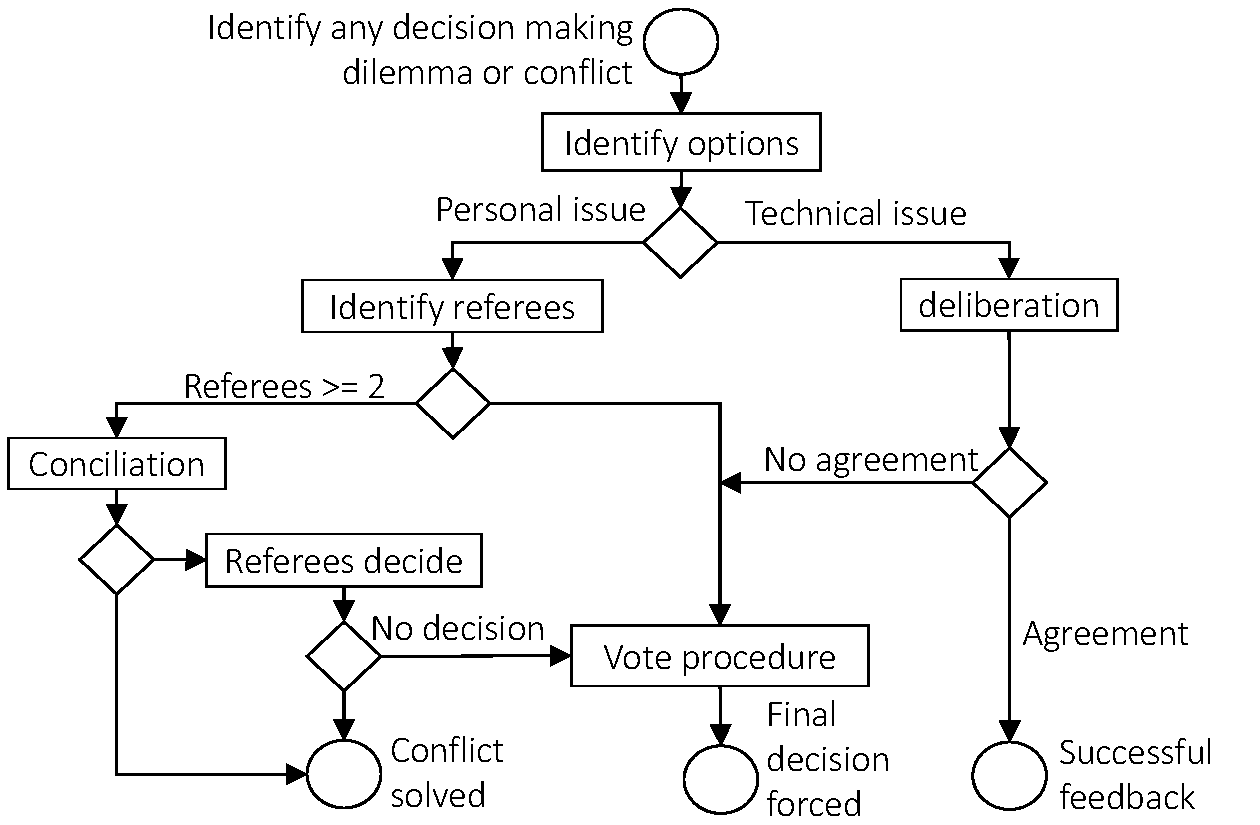
\includegraphics[width=0.6\textwidth]{figs/met}
	\caption{Decision Making and Conflicts Resolution Methodology}
	\label{fig:decisions}
\end{figure}




\subsection{Experiences while working together}

As earlier mentioned, we came from very different backgrounds and we are focusing on different career paths. It's a really good time to become more fluent in Software Engineering. Moreso, most of the industry is moving towards hiring more technically savvy people, that's why some of us picked this module even though it was not mandatory for us.

After learning what the project was going to be about, fortunately, we were interested in the same technologies such as Android and iOS so we split evenly on the different platforms that we were going to use. Each of us picked one technology that we were looking forward to learning in order to succeed in this project. However, that was also enough of a challenge but we succeeded.


For some of us, it was really stressful as we didn't even know how to use the terminal and even struggled with the GitHub command shell. Fortunately, we helped each other a lot and even got a small workshop in which we tested how to work with it.


We had our differences on some meetings. However, we always respected each others points of view and we worked out the overall best solution.
One of the most stressful moment was when we had to decide if we were in fact going to use Firebase. We had our doubts because we were unsure of the NoSQL database. But most of our doubts came from the lack of experience and because we didn't have a clear path towards the goal. We arrived at the conclusion that it is very stressful when you don't have adequate knowledge for the desired goal. 

In order to advance our knowledge as a fast as we could, we first started  reading about chat applications software on GitHub, Coursera, EdX, Udacity, and others.

For the iOS client development, we started with zero experience in Swift and Xcode. We started by building a simple portal to display grades and scores of students of an institution. It also has the feature of adding a new course and grade. With this simple project, we became more confident on developing iOS chat application, at least up to the level shown on this project. Our application was able to meet the requirements listed under our Priority 1 in Table 1 but for how to search for contacts and use Gmail. 
 
Agile Methodology requires dividing the project into small parts so that each part could be tested well before advancing. However, because we needed to learn and develop some skills while implementing, an ideal plan with proper small division was not achieved. 

Above all, we worked together well and we learnt a lot about current technologies and each other's background.

